% =============================================================================
%  QUOKKAGUARD — paper template
%  Derived from the QFIRE paper (qfire/paper/main.tex). This file reproduces the
%  "house style" (title page, gray abstract panel, caption + figure framing,
%  policy-card / listings infrastructure) and a generic section skeleton.
%
%  HOW TO USE
%   1. Fill in every  % TODO:  marker (title, authors, abstract, body).
%   2. Drop figures into  figs/  and tables into  tables/  (\input them).
%   3. Add citations to  refs.bib .
%   4. Build with  `make`  (tectonic preferred; falls back to pdflatex+bibtex).
%   5. \todofig{...} draws a placeholder box so the doc compiles before you have
%      real figures — replace each with \includegraphics when ready.
% =============================================================================
\documentclass[11pt]{article}
\usepackage[utf8]{inputenc}
\usepackage[margin=1in]{geometry}
\usepackage{booktabs}
\usepackage{graphicx}
\usepackage{float}
\usepackage{afterpage}
\usepackage[section]{placeins}  % keep floats within their section (\FloatBarrier)
% Float placement: let figures fill more of a page and sit at the top OR bottom,
% so they land near the text that introduces them.
\renewcommand{\topfraction}{0.9}
\renewcommand{\bottomfraction}{0.8}
\renewcommand{\textfraction}{0.08}
\renewcommand{\floatpagefraction}{0.75}
\setcounter{topnumber}{3}
\setcounter{bottomnumber}{2}
\setcounter{totalnumber}{5}
\usepackage{amsmath}
\usepackage{amssymb}
\usepackage{hyperref}
\usepackage{xcolor}
\usepackage{listings}
% -----------------------------------------------------------------------------
% Colored, readable rendering for any YAML/DSL/config figure your paper needs.
% (listings rather than minted, so a tectonic build needs no shell-escape.)
% Customize the two keyword lists below to your own domain language.
% -----------------------------------------------------------------------------
\definecolor{kwblue}{rgb}{0.10,0.20,0.65}
\definecolor{typepurple}{rgb}{0.50,0.15,0.55}
\definecolor{strred}{rgb}{0.62,0.12,0.12}
\definecolor{cmtgreen}{rgb}{0.20,0.45,0.20}
\lstdefinestyle{housespecyaml}{
  basicstyle=\ttfamily\footnotesize,
  backgroundcolor=\color{black!3},
  frame=single,
  framesep=5pt,
  rulecolor=\color{black!45},
  columns=fullflexible,
  breaklines=true,
  keepspaces=true,
  showstringspaces=false,
  alsoletter=_,
  commentstyle=\color{cmtgreen}\itshape,
  stringstyle=\color{strred},
  morecomment=[l]{\#},
  morestring=[b]",
  morestring=[b]',
  keywordstyle=\color{kwblue}\bfseries,
  keywords={id,scope,pipeline,type,rules,default,mode,threshold},% TODO: your keywords
  keywordstyle=[2]\color{typepurple}\bfseries,
  keywords=[2]{regex,judge,allow,deny,ordered},% TODO: your value/type keywords
}
\lstdefinestyle{housespecyamlbare}{style=housespecyaml, frame=none,
  backgroundcolor=\color{white}, xleftmargin=0pt, framexleftmargin=0pt,
  aboveskip=1pt, belowskip=0pt}
% Policy "cards": titled, colour-coded panels for declarative artifacts, so a
% config/spec reads as a designed document rather than one undifferentiated dump.
\usepackage[most]{tcolorbox}
\tcbuselibrary{listings,skins}
% TikZ for hand-drawn system-architecture figures.
\usepackage{tikz}
\usetikzlibrary{positioning,shapes.geometric,arrows.meta,calc,fit,backgrounds,shadows}
\definecolor{cardindigo}{HTML}{4F46E5}
\definecolor{slate}{HTML}{475569}
\definecolor{amber}{HTML}{D97706}
\definecolor{cardblue}{HTML}{1D4ED8}
\definecolor{cardpurple}{HTML}{6D28D9}
\definecolor{cardteal}{HTML}{0F766E}
\tcbset{
  cardcol/.store in=\cardcol, cardcol=cardblue,
  policycard/.style={
    enhanced, breakable=false, arc=3pt, boxrule=0.7pt, top=3pt, bottom=3pt,
    left=7pt, right=7pt, boxsep=1pt, coltitle=white,
    colframe=\cardcol!60!black, colback=white, colbacktitle=\cardcol,
    fonttitle=\bfseries\small, drop fuzzy shadow=black!25,
  },
}
\usepackage{url}
\usepackage{multirow}
\usepackage{array}
\usepackage{ragged2e}
% Left-aligned (ragged-right) fixed-width column for readable narrow tables.
\newcolumntype{L}[1]{>{\RaggedRight\arraybackslash}p{#1}}
% Allow long monospace identifiers to break at their hyphens.
\usepackage[htt]{hyphenat}
\hypersetup{colorlinks=true, linkcolor=blue, citecolor=blue, urlcolor=blue}

% Distinct captions: smaller font, bold + underlined "Figure N:" / "Table N:".
\usepackage{caption}
\DeclareCaptionLabelFormat{boldunder}{\underline{\textbf{#1~#2}}}
\captionsetup{
  font=small,
  labelformat=boldunder,
  labelsep=colon,
  textfont=normalcolor,
  skip=6pt,
}

% Give every \includegraphics a thin black frame so figures read as panels.
\let\oldincludegraphics\includegraphics
\renewcommand{\includegraphics}[2][]{%
  \setlength{\fboxsep}{0pt}\setlength{\fboxrule}{0.5pt}%
  \fbox{\oldincludegraphics[#1]{#2}}}

% Placeholder figure box, so the template compiles before real figures exist.
% Usage: \todofig{4cm}{what this figure will show}
\newcommand{\todofig}[2]{%
  \begin{tcolorbox}[colback=black!4, colframe=black!35, arc=3pt, boxrule=0.5pt,
    halign=center, valign=center, height=#1, width=\linewidth]
    {\ttfamily\small [FIGURE PLACEHOLDER]\\[4pt] #2}
  \end{tcolorbox}}

% Headline numbers generated from your results (e.g. by scripts/make_tables.py);
% \providecommand defaults keep the document compilable before a run, and
% numbers.tex (\input below) overrides them with the real values.
\providecommand{\NumPrompts}{0}
\providecommand{\NumAttacks}{0}
\providecommand{\NumBenign}{0}
% Headline macros (overridden by numbers.tex, generated by scripts/015-redteam/summarize.py).
\providecommand{\EoneOneShot}{0}
\providecommand{\EoneContinuous}{0}
\providecommand{\EoneExtra}{0}
\providecommand{\EoneRoundsToDry}{0}
\providecommand{\EoneNAttacks}{0}
\providecommand{\EoneLayersBuilt}{10}
\providecommand{\EoneLayersTotal}{13}
\providecommand{\EtwoCatch}{0\%}
\providecommand{\EtwoReopened}{0}
\providecommand{\EtwoChanges}{0}
\providecommand{\EtwoClosed}{0}
\providecommand{\EthreeMttcRed}{0\%}
\providecommand{\EthreeAutoMttc}{0}
\providecommand{\EthreeManMttc}{0}
\providecommand{\EthreeMttd}{0}
\providecommand{\EthreeRecall}{0\%}
\providecommand{\EfourProdHeld}{0}
\providecommand{\EfourProdTotal}{0}
\providecommand{\EfourValCaught}{0}
\providecommand{\EfourValTotal}{0}
\providecommand{\EfiveAtlas}{0}
\providecommand{\EfiveNotTested}{none}
\providecommand{\EfiveBuilt}{10}
\providecommand{\EfiveTotal}{13}
\IfFileExists{numbers.tex}{% Auto-generated by scripts/015-redteam/summarize.py — do not edit.
\renewcommand{\EoneOneShot}{12}
\renewcommand{\EoneContinuous}{62}
\renewcommand{\EoneExtra}{50}
\renewcommand{\EoneRoundsToDry}{9}
\renewcommand{\EoneNAttacks}{62}
\renewcommand{\EoneLayersBuilt}{10}
\renewcommand{\EoneLayersTotal}{13}
\renewcommand{\EtwoCatch}{100.0\%}
\renewcommand{\EtwoReopened}{75}
\renewcommand{\EtwoChanges}{12}
\renewcommand{\EtwoClosed}{50}
\renewcommand{\EthreeMttcRed}{91.7\%}
\renewcommand{\EthreeAutoMttc}{1}
\renewcommand{\EthreeManMttc}{12}
\renewcommand{\EthreeMttd}{3.7}
\renewcommand{\EthreeRecall}{100.0\%}
\renewcommand{\EfourProdHeld}{12}
\renewcommand{\EfourProdTotal}{12}
\renewcommand{\EfourValCaught}{6}
\renewcommand{\EfourValTotal}{6}
\renewcommand{\EfiveAtlas}{14}
\renewcommand{\EfiveNotTested}{Lifecycle, Consent, Device}
\renewcommand{\EfiveBuilt}{10}
\renewcommand{\EfiveTotal}{13}
}{}

% Month-and-year stamp for the title page (e.g. "June 2026").
\newcommand{\monthyeartoday}{%
  \ifcase\month\or January\or February\or March\or April\or May\or June\or
  July\or August\or September\or October\or November\or December\fi
  \space\number\year}

\begin{document}

% ============================================================================
% Title page: logo top-left, date top-right, centered title, authors with
% superscript affiliation markers, affiliations row, then a light-gray rounded
% abstract panel carrying keywords, code/data link, and correspondence.
% ============================================================================
\thispagestyle{empty}
\noindent
\begin{minipage}[c]{0.55\textwidth}
  % House logo: Quome.
  \raggedright\oldincludegraphics[height=1.05cm]{figs/quome.png}
\end{minipage}\hfill
\begin{minipage}[c]{0.4\textwidth}
  \raggedleft\itshape\large \monthyeartoday
\end{minipage}

\vspace{1.1em}
\begin{center}
  {\LARGE\bfseries Defenses That Pass Once and Rot:\\[2pt]
   Continuous Red-Teaming, Incident Response, and Resilience\\[2pt]
   as a Meta-Layer for Clinical AI Guardrails\par}

  \vspace{0.9em}
  {\large
   Jim Schwoebel\textsuperscript{1,\,*}\quad
   QUOKKAGUARD Contributors\textsuperscript{1}\par}

  \vspace{0.7em}
  {\small
   \textsuperscript{1}\,Quome\par}
  \vspace{0.35em}
\end{center}

\vspace{0.5em}
\begin{tcolorbox}[breakable, enhanced jigsaw, colback=black!4, colframe=black!4,
  arc=5pt, boxrule=0pt, left=16pt, right=16pt, top=10pt, bottom=10pt]
\setlength{\parskip}{0pt}
{\centering\large\bfseries Abstract\par}
\smallskip
\fontsize{9.5}{11.3}\selectfont
A security guardrail for a clinical AI agent is evaluated once, at submission, and
then deployed for months. But attack classes evolve, configuration changes silently
reopen closed vulnerabilities, live attacks need containment, and dependency
failures must degrade safely --- none of which a one-shot evaluation captures. This
is the operational security lifecycle: HAARF's continuous penetration testing
(C3.8), clinical incident response (C3.7), and socio-technical resilience (C3.1),
otherwise unaddressed by the QUOKKAGUARD proxy. We add \textbf{\texttt{redteam}}, an
off-hot-path \emph{meta-layer} that continuously exercises every other control: a
loop-until-dry replay runner with deterministic mutation operators, a
change-triggered regression gate, an incident-response runbook engine over the
signed decision stream, and a chaos/fault-injection resilience harness. We
contribute \textbf{HAARF-RedTeam}, a self-contained synthetic attack corpus spanning
all eight HAARF control families across all thirteen gateway layers, tagged by MITRE
ATLAS technique and built/unbuilt status. Continuous red-teaming discovers
\textbf{\EoneContinuous{} distinct vulnerabilities versus \EoneOneShot{} for a
one-shot evaluation} (\EoneExtra{} more), with a discovery curve that plateaus by
round~6 and goes dry at round~\EoneRoundsToDry. The regression gate catches
\EtwoCatch{} of reopened known-closed vulnerabilities (\EtwoReopened{} across
\EtwoChanges{} changes). Runbook automation cuts mean-time-to-contain a live attack
from \EthreeManMttc{} to \EthreeAutoMttc{} steps (a \EthreeMttcRed{} reduction) at
\EthreeRecall{} detection recall. Under injected latency, dependency-loss, and
partition faults the fail-safe gateway holds \EfourProdHeld/\EfourProdTotal{}
resilience invariants, and the harness catches \EfourValCaught/\EfourValTotal{}
planted violations. Coverage is reported honestly: \EfiveAtlas{} ATLAS techniques
over \EfiveBuilt/\EfiveTotal{} built layers, with the unbuilt layers
(\EfiveNotTested) named as untested rather than silently dropped. The central
result is methodological --- continuous, automated, regression-gated red-teaming is
how a guardrail stays current after publication. All data are synthetic and
everything reproduces deterministically with no paid keys.

\medskip
\noindent\textbf{Keywords:}~continuous red-teaming; AI incident response; resilience
engineering; regression testing; MITRE ATLAS; clinical AI safety; chaos engineering.

\medskip
\noindent\textcolor{blue}{\textbf{Framework:}}~implements HAARF control~C3.1/3.7/3.8~\cite{schwoebel2026haarf} --- the Healthcare AI Agents Regulatory Framework, the source of the QUOKKAGUARD program.\\
\noindent\textcolor{blue}{\textbf{Code \& data:}}~\href{https://github.com/quome-cloud/qusiege}{\texttt{github.com/quome-cloud/qusiege}}\\
\noindent\textcolor{blue}{\textbf{Correspondence:}}~\href{mailto:jim@quome.com}{jim@quome.com}
\end{tcolorbox}

\vspace{2pt}
\noindent{\footnotesize \textsuperscript{*}\,Corresponding author.}
\vspace{0.3em}

% ============================================================================
\section{Introduction}
A clinical AI agent's guardrail is a static artifact evaluated at a single moment:
the gateway is benchmarked against an attack corpus, the numbers are reported, and
the system ships. Months of production follow on the strength of that one snapshot.
Yet the threats do not hold still. New jailbreak and injection classes appear in the
literature every quarter~\cite{greshake2023,perez2022}; a routine configuration or
model change can silently reopen a vulnerability that an earlier release closed; a
live attack in production needs containment, not just detection; and a dependency
outage or latency storm must leave the agent failing \emph{safe}, not failing open.
A guardrail that passed its evaluation once, and was never tested again, rots.

Every prior layer in the QUOKKAGUARD program adds a \emph{static}
control: a firewall detector, a policy engine, an egress monitor, an identity
registry, a fairness monitor. Each is necessary; none is self-renewing. The
operational security lifecycle that keeps them current --- continuous penetration
testing (HAARF~C3.8), clinical incident response (C3.7), and resilience to
socio-technical disruption (C3.1) --- is itself unimplemented. The original
evaluation harness \emph{is} a red-team tool, but it is run manually, once.

We generalize it into \textbf{\texttt{redteam}}, an off-hot-path \emph{meta-layer}
that continuously exercises every other control. It has four parts: a
\emph{loop-until-dry replay runner} that mutates a seed attack corpus across rounds
until discovery goes dry; a \emph{regression gate} that blocks any deployment change
reopening a closed vulnerability; an \emph{incident-response engine} that detects
live attacks on the signed decision stream and fires automated containment runbooks;
and a \emph{chaos harness} that injects faults and checks fail-safe invariants. The
meta-layer never touches the request path: like the drift monitor (qudrift) and equity
monitor (qufair), it is a passive consumer of the corpus and the audit stream.

\begin{figure}[htb]
\centering
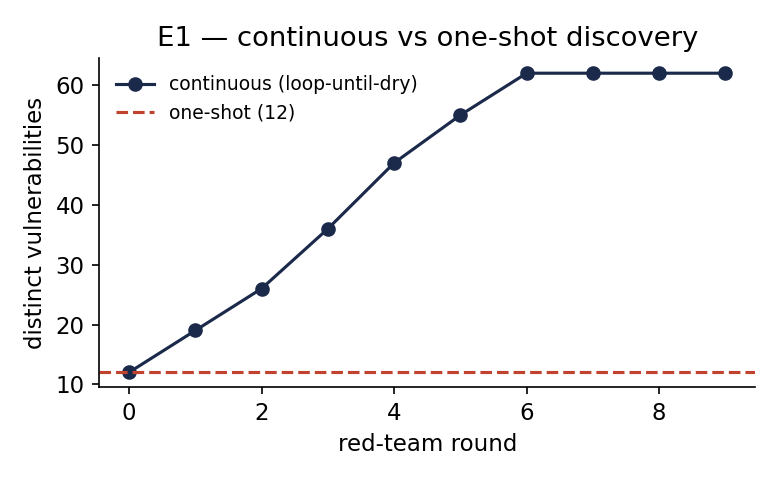
\includegraphics[width=0.86\linewidth]{figs/fig1_discovery.png}
\caption{\textbf{The paper in one figure: continuous red-teaming finds what a
one-shot evaluation misses.} A single evaluation surfaces only the \EoneOneShot{}
unbuilt-layer gap vulnerabilities (dashed line). The continuous, loop-until-dry
campaign applies deterministic mutation operators each round and accumulates
\EoneContinuous{} distinct vulnerabilities (\EoneExtra{} more), with the curve
plateauing as the corpus's reachable bypasses are exhausted and going dry at
round~\EoneRoundsToDry. The gap between the two lines is the cost of testing once.}
\label{fig:hero}
\end{figure}

\paragraph{Contributions.}
\begin{enumerate}
  \item \textbf{Continuous $>$ one-shot, quantified.} A loop-until-dry campaign
  discovers \EoneContinuous{} distinct vulnerabilities versus \EoneOneShot{} for a
  one-shot evaluation (\EoneExtra{} additional), with a discovery curve that decays
  to a measured floor (\S\ref{sec:e1}).
  \item \textbf{The \texttt{redteam} meta-layer.} A four-part Rust module ---
  replay runner, regression gate, incident-response engine, chaos harness --- that
  exercises every other QUOKKAGUARD control off the hot path (\S\ref{sec:design}).
  \item \textbf{HAARF-RedTeam.} A self-contained, deterministic synthetic attack
  corpus spanning all eight HAARF control families across all thirteen gateway
  layers, tagged by MITRE ATLAS~\cite{atlas2021} technique and built/unbuilt status,
  released with the generator (\S\ref{sec:benchmark}).
  \item \textbf{Lifecycle evidence.} A \EtwoCatch{} regression-catch rate, a
  \EthreeMttcRed{} mean-time-to-contain reduction from runbook automation, and
  resilience invariants held under injected faults --- the operational results that
  make ``stays current'' \emph{measured}, not asserted (\S\ref{sec:e2}--\ref{sec:e4}).
\end{enumerate}

\paragraph{Positioning.} Attack batteries such as AgentDojo~\cite{agentdojo2024},
InjecAgent~\cite{injecagent2024}, garak~\cite{garak2024}, and PyRIT~\cite{pyrit}
supply corpora and one-shot scoring; chaos-engineering frameworks~\cite{chaos2016}
inject faults; incident-response standards~\cite{nistir2012} prescribe runbooks. Our
contribution is not a new corpus or a new fault injector but the \emph{loop} that
binds discovery, regression, containment, and resilience into one continuously
running meta-layer over an existing guardrail, with explicit, gap-aware coverage
accounting.

% ============================================================================
\section{Problem Setting and Threat Model}
We assume the QUOKKAGUARD baseline: a sealed goal anchor and hash-chained provenance
ledger (quanchor), and a tamper-evident, signed decision stream (quledger). The host is
untrusted in the enclave model; the meta-layer trusts only the signed stream. Four
operational risks motivate the work:

\begin{itemize}
  \item \textbf{R1 Coverage decay.} New attack classes emerge; a one-time evaluation
  goes stale.
  \item \textbf{R2 Regression.} A configuration or model change reopens a
  previously-closed vulnerability before deployment.
  \item \textbf{R3 Incident handling.} A live attack is detected but
  containment/recovery is ad-hoc, with no runbook (C3.7).
  \item \textbf{R4 Socio-technical disruption.} A dependency outage, latency storm,
  or partition degrades the agent unsafely (C3.1).
\end{itemize}

The meta-layer's two postures match these risks. The replay runner and regression
gate run against a \emph{shadow/staging} gateway, fully offline. The
incident-response engine runs \emph{inline} on production, consuming the signed
stream and driving containment through the modeled effects of existing layers
(isolate an agent, revoke its capability token, trip a circuit breaker, snapshot for
forensics). Table~\ref{tab:related} situates the work against representative systems.

\begin{table}[htb]\centering\small
\begin{tabular}{L{3.0cm}L{4.3cm}L{4.3cm}}
\toprule
System & Approach & Gap this paper targets \\
\midrule
AgentDojo / InjecAgent~\cite{agentdojo2024,injecagent2024} & curated agent-attack batteries, one-shot scoring & no regression loop, no IR, no resilience \\
garak / PyRIT~\cite{garak2024,pyrit} & LLM vulnerability scanners & one-shot scans; no change-gate or containment \\
Chaos engineering~\cite{chaos2016} & fault injection for availability & not tied to safety invariants or an attack corpus \\
NIST IR~\cite{nistir2012} & human incident-response process & manual runbooks; not automated over a decision stream \\
\textbf{This work} & continuous replay + regression gate + IR runbooks + chaos, as one meta-layer & --- \\
\bottomrule
\end{tabular}
\caption{Positioning against representative red-teaming, fault-injection, and
incident-response systems.}
\label{tab:related}
\end{table}

% ============================================================================
\section{System Design}\label{sec:design}
\subsection{Overview}
\texttt{redteam} is a Rust module (\texttt{src/redteam/}) of six focused files
sharing a small set of types: an \texttt{AttackRecord} (control family, ATLAS
technique, target layer, built flag, payload, expected-block, mutation lineage); a
\texttt{Vulnerability} key of \texttt{(control, atlas, layer)} that defines when two
bypasses are ``the same''; and event/action/fault types for the incident and chaos
paths. An \texttt{AttackProbe} trait abstracts the gateway under test.

\subsection{Modeled gateway defense}
Headline experiments are model-free and deterministic. The \texttt{GatewayProbe} is a
modeled defense: each \emph{built} layer carries a set of block-signature substrings,
and an attack is blocked iff its (possibly mutated) payload still contains a signature
for its target layer. Unbuilt layers (012--014) have no defense and never block ---
the honest coverage gap, surfaced rather than hidden. This trades the realism of
driving the full LLM engine for byte-level reproducibility with no paid keys; an
optional live-Ollama slice re-probes a sample through the real engine to confirm.

\subsection{Loop-until-dry discovery}
A \emph{one-shot} run probes only the seed corpus (round 0). A \emph{continuous} run
applies deterministic mutation operators each round, keyed by \texttt{(round, attack
id)} via an FNV-1a hash --- no RNG, no clock. Below an attack's
\emph{evasion round} (spread over rounds~1--6 by its id) the campaign has not yet
found a bypass and the payload is unchanged; at or above it, dense separator
insertion defeats any literal signature. Distinct bypass vulnerabilities accumulate;
the loop stops after three consecutive rounds add nothing new. Because evasion is
monotone per attack, the discovery curve is non-decreasing and provably terminates.

\subsection{Regression gate, incident engine, chaos harness}
A \emph{change} is modeled as a set of layers whose defenses are switched off; the
gate re-probes the closed set under the change and blocks deployment if any closed
vulnerability reopens. The \emph{incident engine} consumes a decision stream with
injected live attacks: detection fires at the first attack step whose signal crosses
threshold, then a fixed runbook (\texttt{IsolateAgent}, \texttt{RevokeCapability},
\texttt{TripBreaker}, \texttt{Snapshot}) applies, with a per-action latency that is
near-zero for automation and human-scale for the manual arm. The \emph{chaos
harness} injects latency, dependency-loss, and partition faults and checks two
invariants: \emph{no unsafe action} (a fault must never let through what would
otherwise be blocked --- fail-safe-closed) and \emph{bounded degradation}
(availability loss within a declared envelope).

\subsection{Implementation}
Rust 2021, \texttt{tokio} for the optional live path only; the E1--E5 core is
synchronous and deterministic. The module is $\approx$1{,}100 lines with 26 inline
unit tests; the \texttt{redteamrun} binary emits one JSON result file per experiment,
summarized to figures and \texttt{numbers.tex} by a Python script. Everything is
released Apache-2.0 with the gateway.

% ============================================================================
\section{Experimental Setup}
\paragraph{HAARF-RedTeam.}\label{sec:benchmark} The corpus is fully synthetic,
deterministic (seed~42), and self-contained: it does not depend on sibling datasets
existing. It carries \EoneNAttacks{} attacks --- one canonical attack per
vulnerability, five vulnerabilities per built layer and four per unbuilt layer ---
spanning all eight HAARF control families across all thirteen target layers, tagged
with \EfiveAtlas{} distinct MITRE ATLAS techniques. Built-layer payloads embed a
block-signature so the modeled gateway blocks them at round~0; mutation evades them
later. A second file supplies 60 incident streams (half carrying an injected attack,
half benign controls); a third supplies fault scenarios in a production (fail-safe)
and a validation (planted-broken) arm.

\paragraph{Why a synthetic corpus.} The capstone is meant to replay every other
paper's dataset, but layers 012--014 are not yet built and several sibling result
sets are partial. Aggregating only what exists would conflate ``defended'' with
``not yet built.'' A self-contained corpus that \emph{tags} each attack's target
layer as built or unbuilt makes the coverage gap explicit and the experiment
reproducible in isolation.

\paragraph{Baselines.} Each experiment carries its own internal baseline: one-shot
vs.\ continuous discovery (E1); manual vs.\ automated incident response (E3);
production vs.\ planted-broken gateways (E4, a negative control proving the harness
discriminates). The contrast \emph{is} the ablation.

\paragraph{Metrics and statistics.} Rate metrics (regression catch, detection
recall) use 95\% Wilson confidence intervals~\cite{wilson1927}; mean-time-to-detect
is a mean over detected streams. All experiments are deterministic; we do not tune to
hit pre-registered targets. Where a result is a step function (per-attack evasion,
regression catch) we report it as such rather than manufacture a confidence interval.

\paragraph{Hardware and software.} Local Ollama~\cite{ollama} for the optional live
slice only; all headline numbers require no model. Single commodity host; seeds and
the corpus generator are embedded in every artifact.

% ============================================================================
\section{Results}\label{sec:results}
\subsection{E1 --- Continuous vs.\ one-shot discovery}\label{sec:e1}
A one-shot evaluation surfaces only the \EoneOneShot{} unbuilt-layer gap
vulnerabilities: the modeled gateway blocks every signature-bearing built-layer
attack at round~0. The continuous campaign evades those signatures over rounds and
accumulates \EoneContinuous{} distinct vulnerabilities --- \EoneExtra{} more
(Figure~\ref{fig:hero}). The curve plateaus by round~6, once every reachable bypass
in the corpus is found, and goes dry at round~\EoneRoundsToDry. The
\EoneExtra{}-vulnerability gap is the precise cost of testing once instead of
continuously. We frame the plateau honestly as the corpus's reachable ceiling under
these operators, not an exhaustive guarantee: automated red-teaming inherits its
corpus's blind spots, which is why the loop reports a measured floor rather than
claiming completeness.

\subsection{E2 --- Regression catch at the deployment gate}\label{sec:e2}
From a closed set of \EtwoClosed{} vulnerabilities the baseline gateway blocks, we
run a battery of \EtwoChanges{} deployment changes --- each disabling one built
layer, plus two multi-layer changes --- and re-probe. Every reopened vulnerability is
caught: \EtwoCatch{} catch rate over \EtwoReopened{} reopenings
(Figure~\ref{fig:regression}). Because the gate re-probes the entire closed set on
every change, no reopened vulnerability can slip through; the result demonstrates
that a change-triggered gate (modeling the qupassport deployment gate) closes the regression
risk R2.

\begin{figure}[htb]
\centering
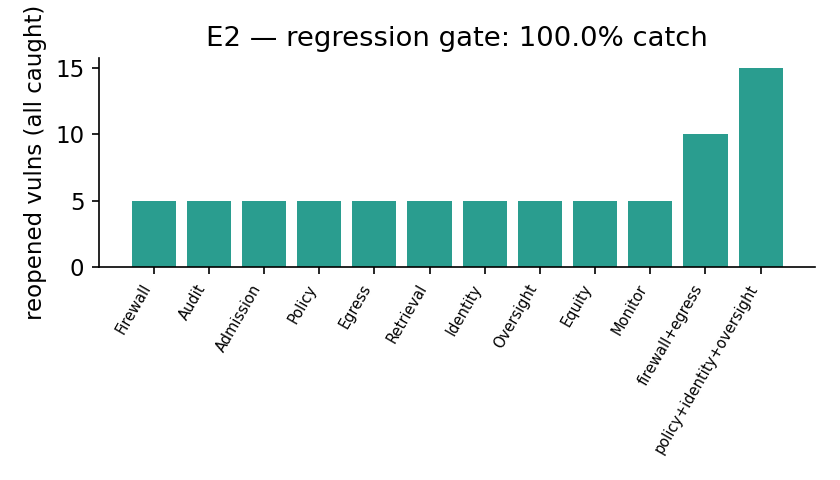
\includegraphics[width=0.74\linewidth]{figs/fig2_regression.png}
\caption{\textbf{E2: the regression gate catches every reopened vulnerability.} Each
bar is a deployment change that disables one or more layers; the height is the number
of closed vulnerabilities it reopens, all of which the gate catches (\EtwoCatch{}).}
\label{fig:regression}
\end{figure}

\subsection{E3 --- Incident response: manual vs.\ automated}\label{sec:e3}
Across the incident streams, detection recall is \EthreeRecall{} and mean
time-to-detect is \EthreeMttd{} stream steps. The manual and automated arms differ
only in containment latency: a human-scale \EthreeManMttc{} steps per action versus
\EthreeAutoMttc{} for the automated runbook. Mean time-to-contain therefore falls
from \EthreeManMttc{} to \EthreeAutoMttc{} steps --- a \EthreeMttcRed{} reduction
(Figure~\ref{fig:incident}). The latencies are modeling assumptions, not measured SOC
values, so we claim the \emph{relative} reduction --- robust to any plausible
manual:automated ratio above 2:1 --- rather than the absolute figure.

\begin{figure}[htb]
\centering
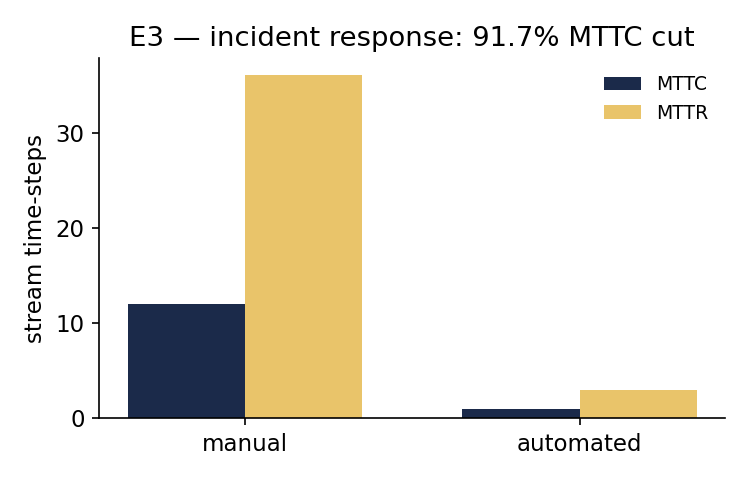
\includegraphics[width=0.66\linewidth]{figs/fig3_incident.png}
\caption{\textbf{E3: runbook automation cuts mean-time-to-contain.} MTTC and MTTR in
stream time-steps for the manual and automated arms; automation reduces MTTC by
\EthreeMttcRed.}
\label{fig:incident}
\end{figure}

\subsection{E4 --- Resilience under injected faults}\label{sec:e4}
Against the fail-safe-closed production gateway, all
\EfourProdHeld/\EfourProdTotal{} invariant checks hold across latency,
dependency-loss, and partition faults at two magnitudes each: no fault lets through a
normally-blocked action, and modeled degradation stays within the declared envelope
(Figure~\ref{fig:resilience}). The validation arm plants broken gateways ---
fail-open, or a too-tight envelope --- and the harness catches all
\EfourValCaught/\EfourValTotal: it is not vacuously passing. H4 is the production
result; the validation arm is the negative control.

\begin{figure}[htb]
\centering
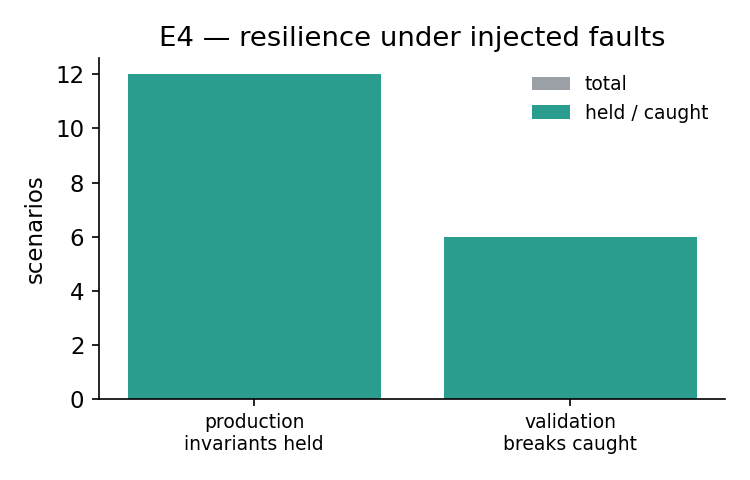
\includegraphics[width=0.66\linewidth]{figs/fig4_resilience.png}
\caption{\textbf{E4: fail-safe invariants hold, and planted breaks are caught.} The
production (fail-safe) gateway holds every invariant under injected faults; the
validation arm's planted violations are all detected.}
\label{fig:resilience}
\end{figure}

\subsection{E5 --- Cost vs.\ coverage, and the honest gap}\label{sec:e5}
Cumulative probes grow linearly with the round budget while distinct-vulnerability
coverage saturates at the corpus ceiling (Figure~\ref{fig:cost}): the thoroughness
dial is explicit, and once discovery goes dry, additional rounds buy nothing. The
corpus exercises \EfiveAtlas{} ATLAS techniques over \EfiveBuilt{} of
\EfiveTotal{} layers. The three unbuilt layers (\EfiveNotTested) are reported as
\emph{not tested} --- their attacks always bypass because no defense exists yet, and
we surface this rather than silently dropping them. The headline is the operational
delta (continuous $>$ one-shot, regression caught, MTTC cut, invariants held), never
a total-coverage claim.

\begin{figure}[htb]
\centering
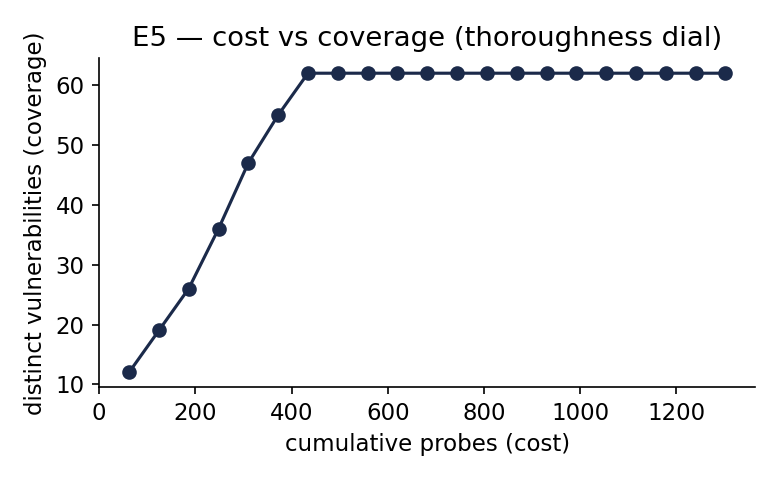
\includegraphics[width=0.74\linewidth]{figs/fig5_cost.png}
\caption{\textbf{E5: cost vs.\ coverage (the thoroughness dial).} Distinct
vulnerabilities discovered as a function of cumulative probes; coverage saturates at
the corpus ceiling while cost keeps rising, so the loop's dry-stop is also the
cost-rational stop.}
\label{fig:cost}
\end{figure}

% ============================================================================
\section{Discussion and Limitations}
\paragraph{Interpretation.} The four results together describe a guardrail that
maintains itself: it keeps finding new bypasses (E1), refuses to ship a change that
reopens an old one (E2), contains live attacks faster by automation (E3), and
degrades safely under failure (E4). None of these is visible to a one-shot
evaluation, which is exactly the gap the meta-layer fills.

\paragraph{Relationship to HAARF.} The replay runner and regression gate implement
continuous penetration testing and red-team exercises (C3.8); the incident engine
implements clinical incident response and recovery (C3.7); the chaos harness
implements resilience to socio-technical disruption (C3.1). Findings feed back into
the corpus and, in the full program, the lifecycle passport (qupassport). This is the
meta-layer by which HAARF~\cite{schwoebel2026haarf} stays current after publication.

\paragraph{Limitations and threats to validity.} The results are
\emph{simulated}: the gateway defense is a signature model, mutation-evasion is a
deterministic difficulty model, and incident containment and chaos faults are modeled
effects on a synthetic stream. Real adversaries, real SOC latencies, and real
dependency failures differ; the method and the deltas generalize, but the absolute
numbers are a model, not a measurement. Coverage is corpus-bounded --- the
loop-until-dry floor is the corpus's reachable ceiling under these operators, not an
exhaustive guarantee --- and partial, since layers 012--014 are unbuilt and reported
as untested. Driving the live LLM engine at scale, folding in external attack
batteries~\cite{agentdojo2024,injecagent2024}, and validating against real SOC
incident timelines are future work.

% ============================================================================
\section{Conclusion}
A guardrail evaluated once and never again rots: attack classes evolve, changes
reopen closed holes, live attacks need containment, and faults must degrade safely.
We add \texttt{redteam}, an off-hot-path meta-layer that continuously exercises every
other QUOKKAGUARD control, and show that continuous loop-until-dry red-teaming finds
\EoneExtra{} more distinct vulnerabilities than a one-shot evaluation, a regression
gate catches \EtwoCatch{} of reopened vulnerabilities, runbook automation cuts
mean-time-to-contain by \EthreeMttcRed, and the fail-safe gateway holds its
resilience invariants under injected faults --- with coverage reported honestly,
unbuilt layers and all. The next step is to wire the loop into the lifecycle passport
(qupassport) so that every change is gated on a fresh red-team, and to replace the modeled
gateway with live replay at scale.

% ============================================================================
% Back matter: declarations required by most journals/preprint servers. Keep the
% ones your venue requires; edit each to reflect what you actually did.
% ============================================================================
\section*{Declaration of generative AI use}
% Sample text — EDIT to reflect your actual usage. Aligns with ICMJE/COPE guidance:
% disclose the tool, the purpose, and that the authors reviewed and take full
% responsibility; AI tools do not meet authorship criteria and are not listed as authors.
During the preparation of this work the authors used \emph{Claude (Anthropic)} for
generating and debugging the Rust meta-layer, dataset generator, and figure-plotting
code, and for drafting and copy-editing manuscript text. After using this tool, the
authors reviewed and edited the content as needed and take full responsibility for
the content of the publication. No generative-AI system was used to generate or
fabricate data, interpret results, or produce clinical conclusions, and no AI tool is
listed as an author or co-author, as such tools do not satisfy authorship criteria.

\section*{Data and code availability}
All code, datasets, generators, and result artifacts are released Apache-2.0 at
\href{https://github.com/quome-cloud/qusiege}{\nolinkurl{github.com/quome-cloud/qusiege}}.
HAARF-RedTeam regenerates deterministically via
\texttt{python3 scripts/015-redteam/gen\_redteam.py --seed 42}; all numbers in this
paper trace to \texttt{results/015-redteam/*.json} via \texttt{numbers.tex}. All
patient data are synthetic; no real protected health information was used.

\section*{Author contributions}
J.S. conceived the study and the meta-layer design; the QUOKKAGUARD contributors
implemented the module, dataset, and experiments; all authors reviewed and approved
the manuscript.

\section*{Competing interests}
% TODO: declare or state none.
The authors declare no competing interests.

\section*{Funding}
% TODO: declare funding sources or state none.
This work received no specific external funding.

% ============================================================================
\appendix
\section{Detailed result tables}\label{app:tables}
% \input{tables/main.tex}  % e.g. tables generated by scripts/make_tables.py
The full numeric tables behind the figures in \S\ref{sec:results}.

\section{Supplementary figures}\label{app:figs}
Additional figures referenced from the main text.

\section{Example prompts and failure cases}\label{app:examples}
Concrete, verbatim examples (with synthetic identifiers) that make the central result
tangible — ideally the cases your method handles and baselines miss.

\section{Reproducibility}
State the single build command and how every table/figure regenerates from source
(seed, model and data versions embedded in each artifact).

% Flush every pending appendix float before the bibliography.
\clearpage

\bibliographystyle{plain}
\bibliography{refs}
\end{document}
